\chapter{Arquitectura del sistema}
\label{ch:arquitectura}

Este capítulo describe la organización estructural del simulador: los componentes que lo forman, cómo se relacionan entre sí y las decisiones de diseño que condicionan esa organización. El detalle de implementación de cada componente se desarrolla en el capítulo~\ref{ch:implementacion}.

El sistema está compuesto por cinco bloques funcionales: una interfaz web, un backend de orquestación, tres instancias del motor de enrutado viario OSRM, un planificador de transporte público basado en OpenTripPlanner y un módulo de inferencia de elección modal. Todos ellos se despliegan como contenedores Docker orquestados mediante Docker Compose.

% -------------------------------------------------------
\section{Visión general}
\label{sec:arch_vision_general}
% -------------------------------------------------------

La Figura~\ref{fig:arch_general} muestra la arquitectura de alto nivel del sistema. El principio de diseño central es que el frontend nunca se comunica directamente con ningún servicio externo: toda petición pasa por el backend de FastAPI, que actúa como única puerta de entrada y punto de orquestación. Esta decisión simplifica el control de versiones de la API, centraliza el manejo de errores y evita exponer los puertos internos de OSRM y OTP al navegador.

\begin{figure}[htbp]
  \centering
  % \includegraphics[width=0.92\textwidth]{figures/arch_general.pdf}
  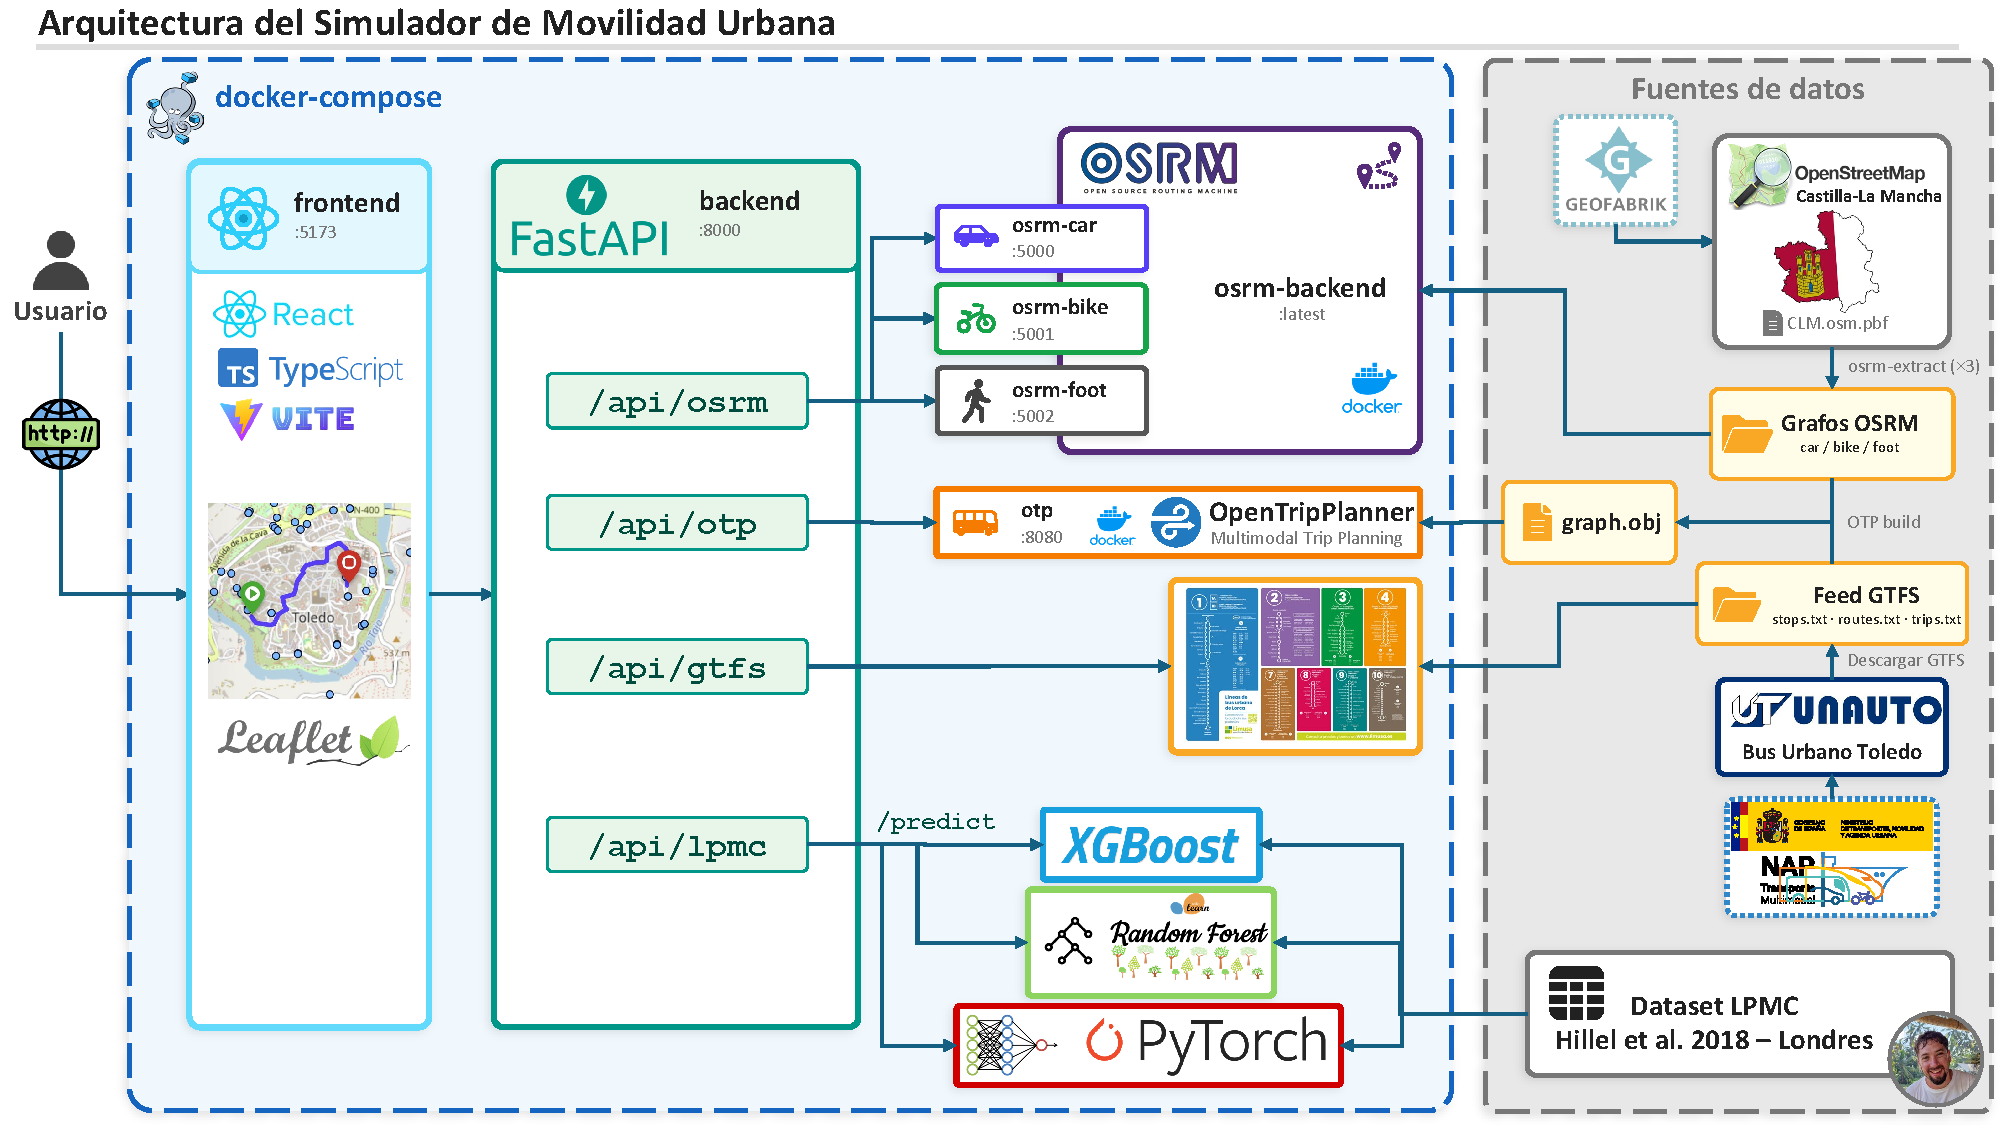
\includegraphics[width=\textwidth]{figs/ARQUITECTURA_pytorch_final.pdf}
  \caption{Arquitectura general del simulador de movilidad urbana.}
  \label{fig:arch_general}
\end{figure}

El frontend expone la interfaz cartográfica al usuario y delega en el backend el cálculo de rutas, la consulta de horarios GTFS y la inferencia modal. El backend integra cuatro routers diferenciados: \texttt{/api/osrm} para rutas viarias por perfil, \texttt{/api/otp} para itinerarios multimodales, \texttt{/api/gtfs} para información estática de la red de transporte, y \texttt{/api/lpmc} para la inferencia de elección modal. Cada router encapsula la lógica de comunicación con su servicio subyacente y expone al frontend una interfaz homogénea independiente de los detalles de cada protocolo.

% -------------------------------------------------------
\section{Infraestructura y orquestación}
\label{sec:arch_infra}
% -------------------------------------------------------

La infraestructura del sistema se define íntegramente en un fichero \texttt{docker-compose.yml} en la raíz del repositorio. El despliegue completo se obtiene con un único comando (\texttt{docker compose up -{}-build}), lo que elimina dependencias de entorno en la máquina anfitriona y garantiza reproducibilidad.

\begin{figure}[htbp]
  \centering
  % \includegraphics[width=0.92\textwidth]{figures/arch_docker.pdf}
  \missingfigure{Diagrama de servicios Docker Compose: frontend :5173, backend :8000, osrm-car :5001, osrm-bike :5002, osrm-foot :5003, otp :8080, y servicios de inicialización gtfs-init, osrm-setup y otp-build. Volúmenes montados en OSRM y OTP.}
  \caption{Servicios Docker Compose y puertos expuestos.}
  \label{fig:arch_docker}
\end{figure}

La Tabla~\ref{tab:servicios_docker} resume los servicios definidos, sus puertos y su función en el sistema.

\begin{table}[htbp]
  \caption{Servicios Docker Compose del simulador.}
  \label{tab:servicios_docker}
  \centering
  \begin{tabular}{llp{7cm}}
    \hline
    \textbf{Servicio} & \textbf{Puerto} & \textbf{Función} \\
    \hline
    \texttt{frontend}   & 5173 & Interfaz web React servida por Vite. \\
    \texttt{backend}    & 8000 & API FastAPI, orquestación y lógica de negocio. \\
    \texttt{osrm-car}   & 5001 & Motor OSRM con perfil de vehículo a motor. \\
    \texttt{osrm-bike}  & 5002 & Motor OSRM con perfil de bicicleta. \\
    \texttt{osrm-foot}  & 5003 & Motor OSRM con perfil peatonal. \\
    \texttt{otp}        & 8080 & OpenTripPlanner 2.x con grafo multimodal de Toledo. \\
    \hline
  \end{tabular}
\end{table}

Los servicios OSRM montan los grafos viarios preprocesados desde directorios locales mediante volúmenes Docker. OpenTripPlanner carga el grafo multimodal (\texttt{graph.obj}) generado a partir de los datos OSM de Castilla-La Mancha y el feed GTFS urbano de Toledo. Estos artefactos pesados se versionan mediante Git LFS (\textit{Large File Storage}), de modo que un clon del repositorio dispone de ellos sin necesidad de reconstruirlos. Para cubrir el caso de un clon sin LFS o de una actualización de los datos de origen, la orquestación incorpora además varios servicios de inicialización idempotentes que se ejecutan una sola vez antes de levantar el sistema: \texttt{gtfs-init} descomprime el feed GTFS, \texttt{osrm-setup} preprocesa los grafos viarios por perfil si faltan y \texttt{otp-build} construye el grafo de OTP si no está presente. El procedimiento completo, tanto automático como manual, se describe en el anexo~\ref{anx:despliegue}.

La razón por la que OSRM se instancia tres veces en lugar de usar un único servidor multiperfil es que la imagen oficial de OSRM no admite perfiles simultáneos: cada proceso solo puede servir el grafo con el que fue preprocesado. Esta limitación fue el detonante del cambio de la solución inicial basada en el servidor de demostración público, que únicamente ofrecía perfil de conducción, a la infraestructura local multiperfil descrita aquí.

% -------------------------------------------------------
\section{Backend: capa de orquestación}
\label{sec:arch_backend}
% -------------------------------------------------------

El backend está implementado con FastAPI sobre Python y se organiza en cuatro routers, cada uno responsable de un dominio funcional. La separación en routers permite desarrollar, probar y documentar cada integración de forma independiente. La Tabla~\ref{tab:endpoints_api} recoge los endpoints principales expuestos por cada router.

\begin{table}[htbp]
  \caption{Endpoints principales de la API REST del backend.}
  \label{tab:endpoints_api}
  \centering
  \begin{tabular}{llp{6.5cm}}
    \hline
    \textbf{Método} & \textbf{Ruta} & \textbf{Descripción} \\
    \hline
    POST & \texttt{/api/osrm/routes}                  & Rutas viarias multimodales (OSRM). \\
    POST & \texttt{/api/otp/routes}                   & Itinerario de transporte público (OTP). \\
    GET  & \texttt{/api/gtfs/stops}                   & Listado de paradas con filtro bbox. \\
    GET  & \texttt{/api/gtfs/routes}                  & Listado de líneas de la red. \\
    GET  & \texttt{/api/gtfs/routes/\{id\}}           & Detalle de ruta: paradas y trazado. \\
    GET  & \texttt{/api/gtfs/routes/\{id\}/schedule}  & Horarios de una línea por fecha. \\
    POST & \texttt{/api/lpmc/predict}                 & Inferencia de elección modal con el modelo activo. \\
    POST & \texttt{/api/lpmc/compare}                 & Inferencia simultánea con XGBoost, RF y DNN. \\
    POST & \texttt{/api/lpmc/debug-features}          & Vector de características antes/después del escalado. \\
    GET  & \texttt{/api/lpmc/models}                  & Modelos disponibles y variante por defecto. \\
    GET  & \texttt{/health}                           & Comprobación de disponibilidad. \\
    \hline
  \end{tabular}
\end{table}

El router \texttt{/api/osrm} recibe un par origen-destino con la lista de perfiles solicitados, consulta en paralelo las instancias OSRM correspondientes y devuelve al frontend las rutas con distancia, duración y geometría decodificada para su representación cartográfica.

El router \texttt{/api/otp} consulta el planificador multimodal y gestiona la paginación de itinerarios alternativos. La respuesta incluye el desglose por tramos (\textit{legs}), con tipo de modo, geometría, parada de inicio y fin, y agencia operadora cuando el tramo es de transporte público. Los itinerarios se ordenan por duración y se selecciona automáticamente el primero que incluya al menos un tramo de transporte público; si ninguno lo incluye, se devuelve el de menor duración.

El router \texttt{/api/gtfs} expone información estática de la red de transporte: listado de paradas con sus líneas asociadas, listado de rutas, detalle de ruta con paradas ordenadas y trazado geométrico, y resumen de horarios por fecha. Estos datos se leen directamente del feed GTFS descomprimido en el backend, sin depender de OpenTripPlanner, lo que permite consultar la red aunque el grafo OTP no esté disponible.

El router \texttt{/api/lpmc} recibe las coordenadas de origen y destino junto con el perfil sociodemográfico del viajero, construye el vector de variables de entrada al modelo consultando OSRM y OTP internamente, convierte las duraciones a horas para coincidir con las unidades del dataset de entrenamiento, aplica el escalado parcial y ejecuta la inferencia. El endpoint \texttt{/predict} usa el modelo activo; \texttt{/compare} ejecuta los tres modelos (XGBoost, Random Forest, DNN) sobre el mismo viaje y devuelve sus probabilidades comparadas; \texttt{/debug-features} expone el vector de características antes y después del escalado para validación del pipeline.

% -------------------------------------------------------
\section{Frontend: interfaz cartográfica}
\label{sec:arch_frontend}
% -------------------------------------------------------

El frontend está desarrollado con React, Vite y TypeScript. La aplicación se estructura en dos componentes principales: \texttt{App}, que concentra el estado global y la lógica de negocio del cliente, y \texttt{MapView}, que encapsula la representación cartográfica mediante React-Leaflet.

\texttt{App} gestiona los puntos de origen y destino, el modo de transporte activo, los resultados de rutas, la capa GTFS y el perfil de usuario para la inferencia. Las peticiones al backend se realizan con TanStack Query (\texttt{useQuery} y \texttt{useMutation}), que proporciona caché, gestión de estados de carga y reintento automático. El estado local de React es suficiente para el alcance del prototipo: no existe flujo de datos compartido entre componentes independientes que justifique una biblioteca adicional de gestión de estado.

\texttt{MapView} recibe el estado relevante como \textit{props} y se encarga exclusivamente de la renderización cartográfica: marcadores de origen y destino, polilíneas de ruta coloreadas según el modo activo, paradas GTFS con popups interactivos y segmentos OTP diferenciados visualmente entre tramos a pie y tramos en vehículo. Los segmentos de transporte público solo se muestran cuando el modo activo es \textit{transit}, evitando solapamientos visuales con las rutas viarias. La capa de fondo es configurable entre cuatro basemaps: carto-light (analítico, sin distracciones visuales), OpenStreetMap estándar (cartografía en color), OpenTopoMap (relieve con curvas de nivel) y satélite Esri (imágenes aéreas).

% -------------------------------------------------------
\section{Pipeline de inferencia modal}
\label{sec:arch_pipeline_inferencia}
% -------------------------------------------------------

La inferencia de elección modal es la operación más compleja del sistema porque requiere coordinar tres servicios externos de forma concurrente para construir el vector de entrada al modelo. La Figura~\ref{fig:pipeline_inferencia} ilustra el flujo completo.

\begin{figure}[htbp]
  \centering
  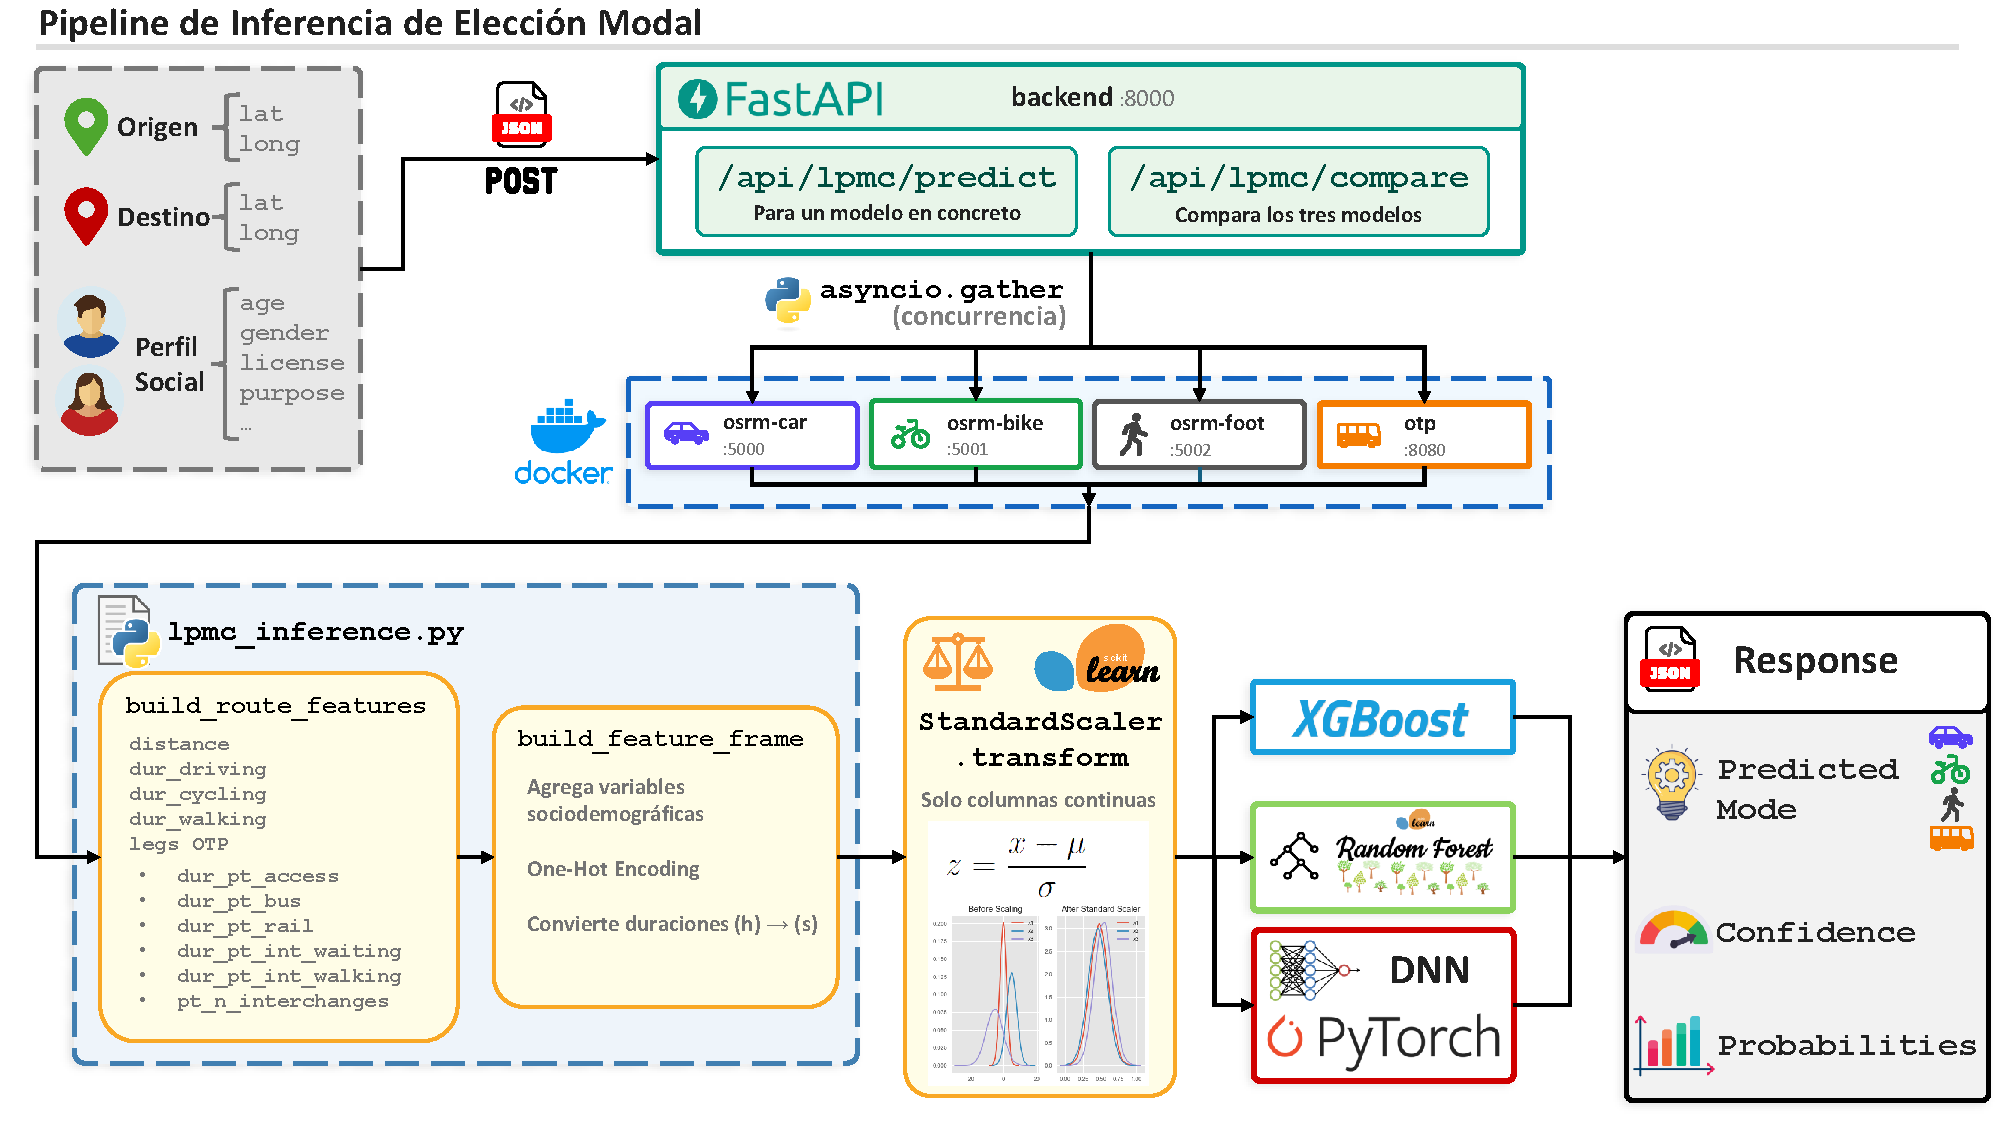
\includegraphics[width=\textwidth]{figs/PIPELINE_Inferencia.pdf}
  \caption{Pipeline de inferencia de elección modal.}
  \label{fig:pipeline_inferencia}
\end{figure}

Al recibir una petición \texttt{POST /api/lpmc/predict}, el backend lanza en paralelo cuatro consultas asíncronas mediante \texttt{asyncio.gather}: una a cada una de las tres instancias OSRM (conducción, bicicleta, a pie) y una a OpenTripPlanner. Con los resultados se construye el vector de características de ruta, se añaden las variables sociodemográficas del perfil recibido en la petición y se ensambla el vector completo de entrada al modelo.

Las variables de entrada al modelo proceden de tres fuentes diferenciadas: los tiempos y distancias por perfil de transporte calculados por OSRM, el desglose temporal del itinerario de transporte público proporcionado por OTP, y los datos sociodemográficos y contextuales que el usuario introduce en el formulario del panel lateral. El capítulo~\ref{ch:implementacion} detalla la construcción del vector de características y las transformaciones aplicadas.

Las variables continuas que presentaban distribución asimétrica en el conjunto de entrenamiento se normalizan con un escalado parcial aplicado solo a las columnas correspondientes, preservando las variables binarias y de conteo sin transformar. El modelo devuelve un vector de cuatro probabilidades correspondientes a los modos \textit{walk}, \textit{cycle}, \textit{pt} y \textit{drive}; el modo predicho es el de mayor probabilidad.

El modelo utilizado en \texttt{/predict} se elige mediante el parámetro opcional \texttt{model\_variant} de la propia petición; cuando no se indica, se recurre a la variable de entorno \texttt{LPMC\_MODEL\_VARIANT} (\texttt{xgb} por defecto), lo que mantiene la compatibilidad con clientes que no especifiquen el modelo. Ninguno de los tres modelos recibe \texttt{household\_id} como variable de entrada, ya que ese identificador de hogar no está disponible en tiempo de ejecución; su uso durante el entrenamiento se detalla en la sección~\ref{subsec:impl_lpmc_entrenamiento}.

% Decisiones técnicas movidas al capítulo 5 (implementación)

% % -------------------------------------------------------
% \section{Decisiones técnicas (ch5)}
% \label{sec:arch_decisiones}
% % -------------------------------------------------------

% A lo largo del desarrollo se tomaron varias decisiones de diseño que condicionan la arquitectura actual.

% \textbf{OSRM local frente al servidor de demostración.} La solución inicial utilizaba el demoserver público de OSRM, que solo proporciona el perfil de conducción. La imposibilidad de obtener tiempos de bicicleta y desplazamiento a pie, variables imprescindibles para el modelo LPMC, obligó a desplegar OSRM localmente con tres perfiles independientes. El coste es un mayor requisito de almacenamiento y memoria en tiempo de ejecución, compensado por la autonomía completa sobre los datos y la ausencia de límites de cuota.

% \textbf{Tres instancias OSRM en lugar de una.} La imagen oficial de OSRM no admite múltiples perfiles en un único proceso: cada instancia solo puede servir el grafo con el que fue preprocesada mediante \texttt{osrm-extract} y \texttt{osrm-partition}. La solución adoptada es desplegar tres contenedores independientes, cada uno con su grafo, mapeados a puertos distintos del host.

% \textbf{Fecha y hora fijas en OTP.} OpenTripPlanner calcula itinerarios en función de los calendarios de servicio del feed GTFS. Usar la fecha y hora reales introducía inconsistencias: en fines de semana o festivos el servicio es reducido o inexistente, lo que hacía que OTP devolviera itinerarios atípicos o ninguno. La solución adoptada es usar una fecha laborable fija (\texttt{2025-12-01}) y una hora de alta frecuencia de servicio (\texttt{12:00}), garantizando resultados representativos del servicio habitual.

% \textbf{Variante nohh del modelo LPMC.} El modelo original incluía \texttt{household\_id} como variable de entrada, lo que imposibilita su uso en inferencia ya que el simulador no tiene acceso a ese identificador. Se entrenó una variante alternativa excluyendo esa variable (\texttt{nohh}), que es la activa por defecto. La variante original se conserva como respaldo y el sistema puede alternar entre ambas mediante variable de entorno.

% \textbf{Colores de línea GTFS deterministas.} El feed GTFS de Toledo no incluye de forma consistente los campos \texttt{route\_color} y \texttt{route\_text\_color}. Para garantizar consistencia visual entre sesiones, el color de cada línea se deriva de forma determinista a partir del \texttt{route\_id} mediante una función de hash, de modo que la misma línea siempre se muestra con el mismo color independientemente del estado del servidor.

% \textbf{Carga perezosa de artefactos del modelo.} Los modelos (XGBoost, Random Forest, DNN) y sus escaladores se cargan desde disco la primera vez que se solicita cada variante y se mantienen en caché indexada por variante a nivel de módulo durante toda la vida del proceso. Esta estrategia de carga perezosa (\textit{lazy loading}) evita aumentar el tiempo de arranque del contenedor y garantiza que cada artefacto se carga exactamente una vez, independientemente del número de peticiones concurrentes.

% \textbf{Penalización de variables PT sin itinerario real.} Cuando OTP no encuentra un itinerario con transporte público, las variables de ruta PT (\texttt{dur\_pt\_access}, \texttt{dur\_pt\_bus}, \texttt{dur\_pt\_rail}, \texttt{pt\_n\_interchanges}) toman valor cero, lo que puede inducir al modelo a predecir \textit{pt} como modo mayoritario en trayectos sin servicio real. La solución, pendiente de implementar en el momento de escritura, consiste en asignar un valor de penalización alto a estas variables cuando OTP no devuelva un itinerario con al menos un tramo de transporte público.